\graphicspath{{../Graphics/Cpt3-CombInject/}}

En este cap\'itulo se han combinado los m\'etodos de generaci\'on de OFC estudiados en los cap\'itulos anteriores, abordando el estudio de los regímenes din\'amicos que existen en la generaci\'on de OFC mediante \gs\ e inyecci\'on de luz. Se ha trabajado con el l\'aser SL con $\ibias = 35$ mA, $V_{RF} = 1.$ V y alta frecuencia $f_R = 5$ GHz. Para las condiciones de inyecci\'on de ML se ha tomado un \'unico valor de $\delta\nu = -2$ GHz, variando la potencia de inyecci\'on $P_{Iny}$.

En la Figura \ref{Img:MapGS-IO} se muestran los espectros \'opticos de las diferentes regiones din\'amicas obtenidas para distintas $P_{Iny}$ a $\delta\nu = -2$ GHz. 

	\begin{figure}[H]
		\centering
		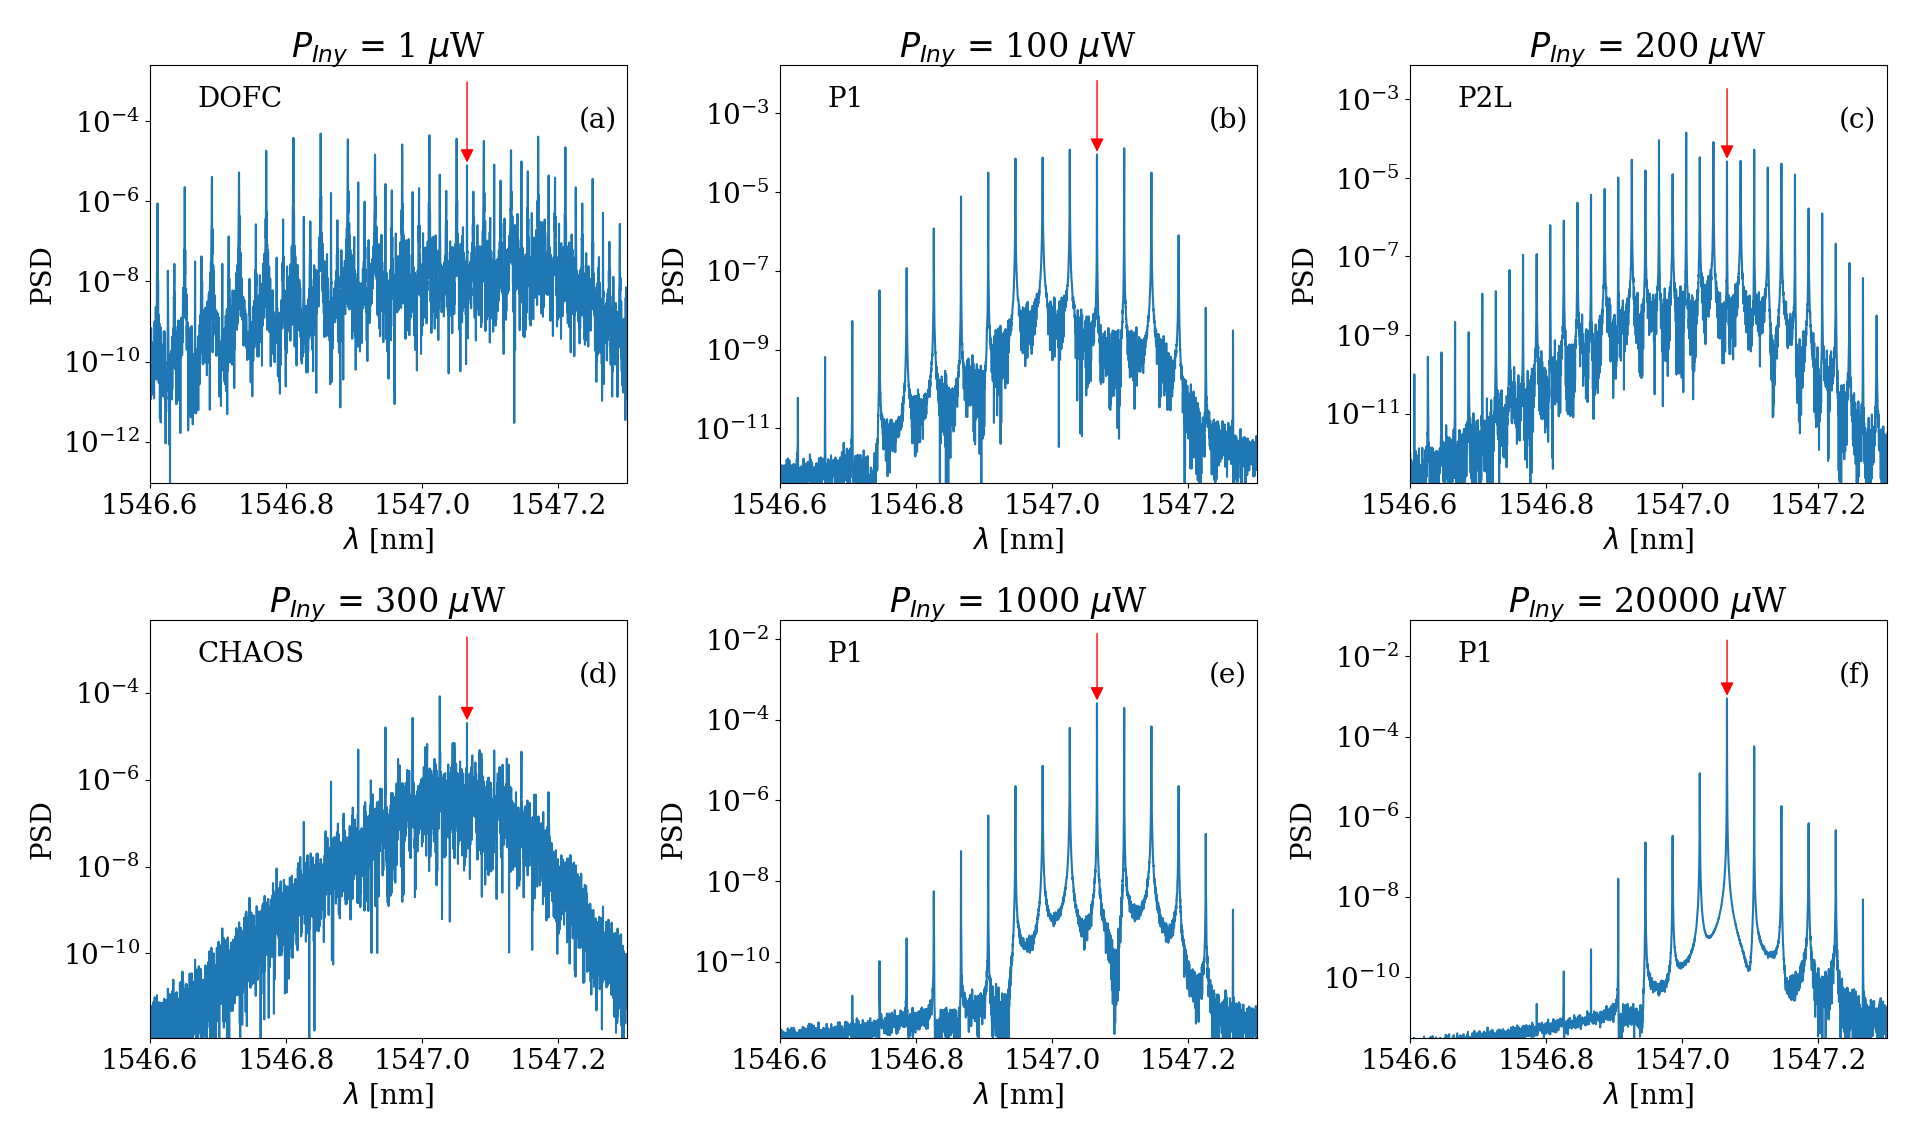
\includegraphics[width=1.0\linewidth]{psdMap.png}
		\caption{\label{Img:MapGS-IO}Espectros \'opticos obtenidos mediante \gs\ e inyección \'optica de las diferentes regiones dinámicas obtenidas para diferentes $P_{Iny}$ a $\delta\nu = -2$ GHz. Se indica la frecuencia de inyección $\nu_{ML}$ con una flecha y $P_{Iny}$ para cada espectro \'optico.}
	\end{figure}

Para $P_{Iny} = 1\;\mu$W se obtiene un espectro \'optico con doble peine \'optico de frecuencias, DOFC (Figura \ref{Img:MapGS-IO} (a)). Este consiste en la superposición de dos peines, el obtenido sin inyección óptica, y el centrado en la frecuecia del láser maestro $\nu_{ML}$, con una separación de frecuencias entre líneas también de $f_R$. El DOFC desaparece al aumentar la potencia de inyección, obteniendo un OFC simple en la regi\'on P1 para $P_{Iny} = 100\;\mu$W (Figura \ref{Img:MapGS-IO} (b)). Este OFC tiene una línea que aparece a $\nu_{ML}$ y la separación entre líneas sigue siendo $f_R$. Al aumentar $P_{Iny} = 200 \;\mu$W se produce un doblamiento de periodo P2, obteniendo un OFC cuyas frecuencias de separaci\'on entre pico es la mitad que para la regi\'on P1 (Figura \ref{Img:MapGS-IO} (c)). La región de caos, CHAOS, se obtiene para $P_{Iny} = 300\;\mu$W, para la que el OFC se destruye (Figura \ref{Img:MapGS-IO} (d)). Con altas potencias de inyecci\'on $P_{Iny} = 1000\;\mu$W y $ 20000\;\mu$W se alcanza nuevamente la regi\'on P1 con un pico m\'aximo para la frecuencia de inyecci\'on $\nu_{ML}$. Dentro de esta regi\'on, al aumentar $P_{Iny}$ tanto el ruido debido a la emisi\'on espont\'anea como el ancho de la envolvente del OFC disminuyen, mientras que el pico con la frecuencia de inyecci\'on aumenta.

Se han estudiado y comparado algunos casos concretos de las regiones mostradas en la Figura \ref{Img:MapGS-IO}, analizando el comportamiento de las variables internas con el objetivo de entender mejor los fen\'omenos que se producen en cada caso, de cara a realizar una correcta distinci\'on de las diferentes regiones din\'amicas.

En la Figura \ref{fig:p1-p2} se muestran los espectros \'opticos, $P(t)$ y la proyecci\'on del atractor en el plano ($N(t)$, $P(t)$) del espacio de estados; para $\delta\nu = -2$GHz y $P_{Iny} = 100\;\mu$W y $200\;\mu$W.

	\begin{figure}[H]
		\centering
		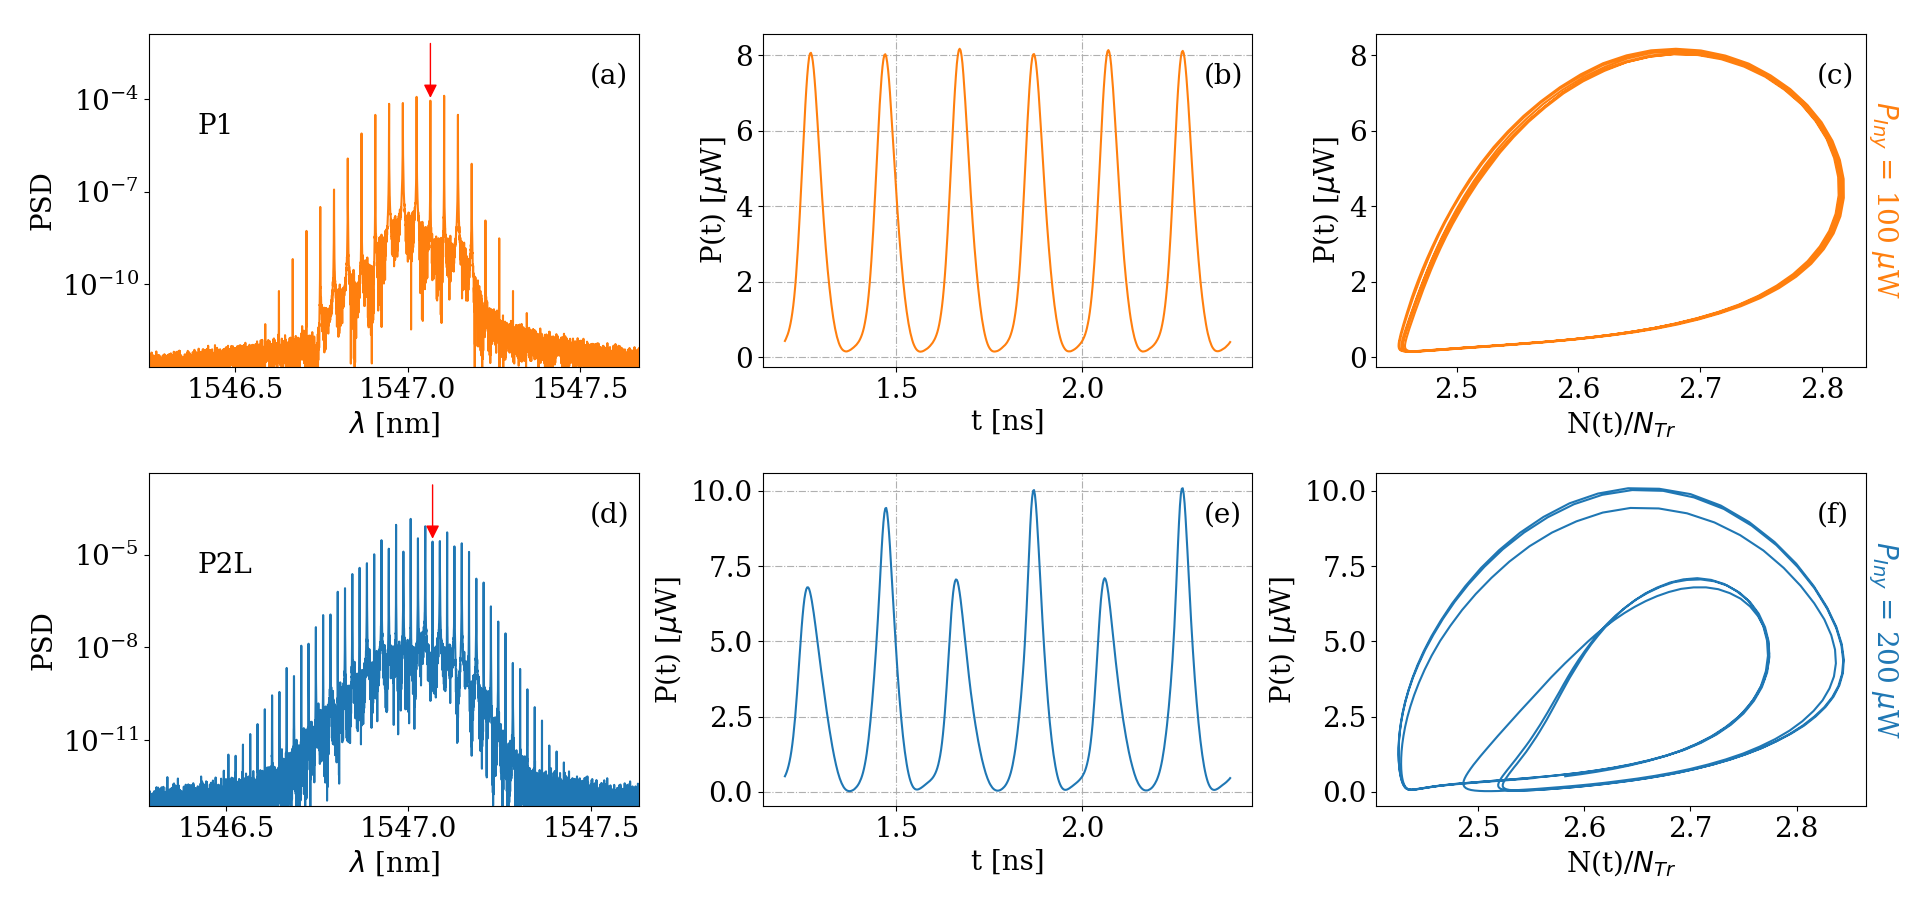
\includegraphics[width=1.0\linewidth]{p1-p2.png}
		\caption{\label{fig:p1-p2}Espectros \'opticos, $P(t)$ y proyecci\'on del atractor en el plano ($N(t)$, $P(t)$) del espacio de estados; para $\delta\nu = -2$GHz y $P_{Iny} = 100\;\mu$W (P1, naranja) y $200\;\mu$W (P2, azul).}	
	\end{figure}

	Los resultados de la Figura \ref{fig:p1-p2} permiten ilustrar la transición entre las soluciones P1 y P2. En el espectro \'optico de $P_{Iny} = 100\;\mu$W (Figura \ref{fig:p1-p2} (a)) se obtiene un OFC cuya separaci\'on entre picos es $\Delta f = 7.5$ GHz, mientras que para el OFC obtenido con $P_{Iny} = 200\;\mu$W (Figura \ref{fig:p1-p2}(d)) la separaci\'on es de $\Delta f = 15$ GHz, siendo el doble, en el dominio de las frecuencias, que en el caso anterior. \'Esto indica como entre las potencias $P_{Iny} = 100\;\mu$W y $200\;\mu$W se van desarrollando picos para la mitad de separación en $\lambdas$. Esto se puede observar en la Figura \ref{fig:p1-p2} (e) en la que la diferencia de amplitudes entre picos consecutivos produce que el periodo de las oscilaciones de $P(t)$ no sea el tiempo entre estos picos, sino el tiempo entre picos con la misma amplitud. Tambi\'en se puede observar en la Figura \ref{fig:p1-p2} (f) en la que se obtiene un lazo extra con un diagrama similar al de la Figura \ref{fig:P2zone} (f) para la regi\'on P2 del c\'apitulo anterior.

FASE AUNQUE NO SE QUE DECIR NI SI AQUI ES EL MEJOR SITIO

En la Figura \ref{fig:chaos} se muestran los espectros \'opticos, $P(t)$ y la proyecci\'on del atractor en el plano ($N(t)$, $P(t)$) del espacio de estados; para $\delta\nu = -2$GHz y $P_{Iny} = 1\;\mu$W y $300\;\mu$W.

	\begin{figure}[H]
		\centering
		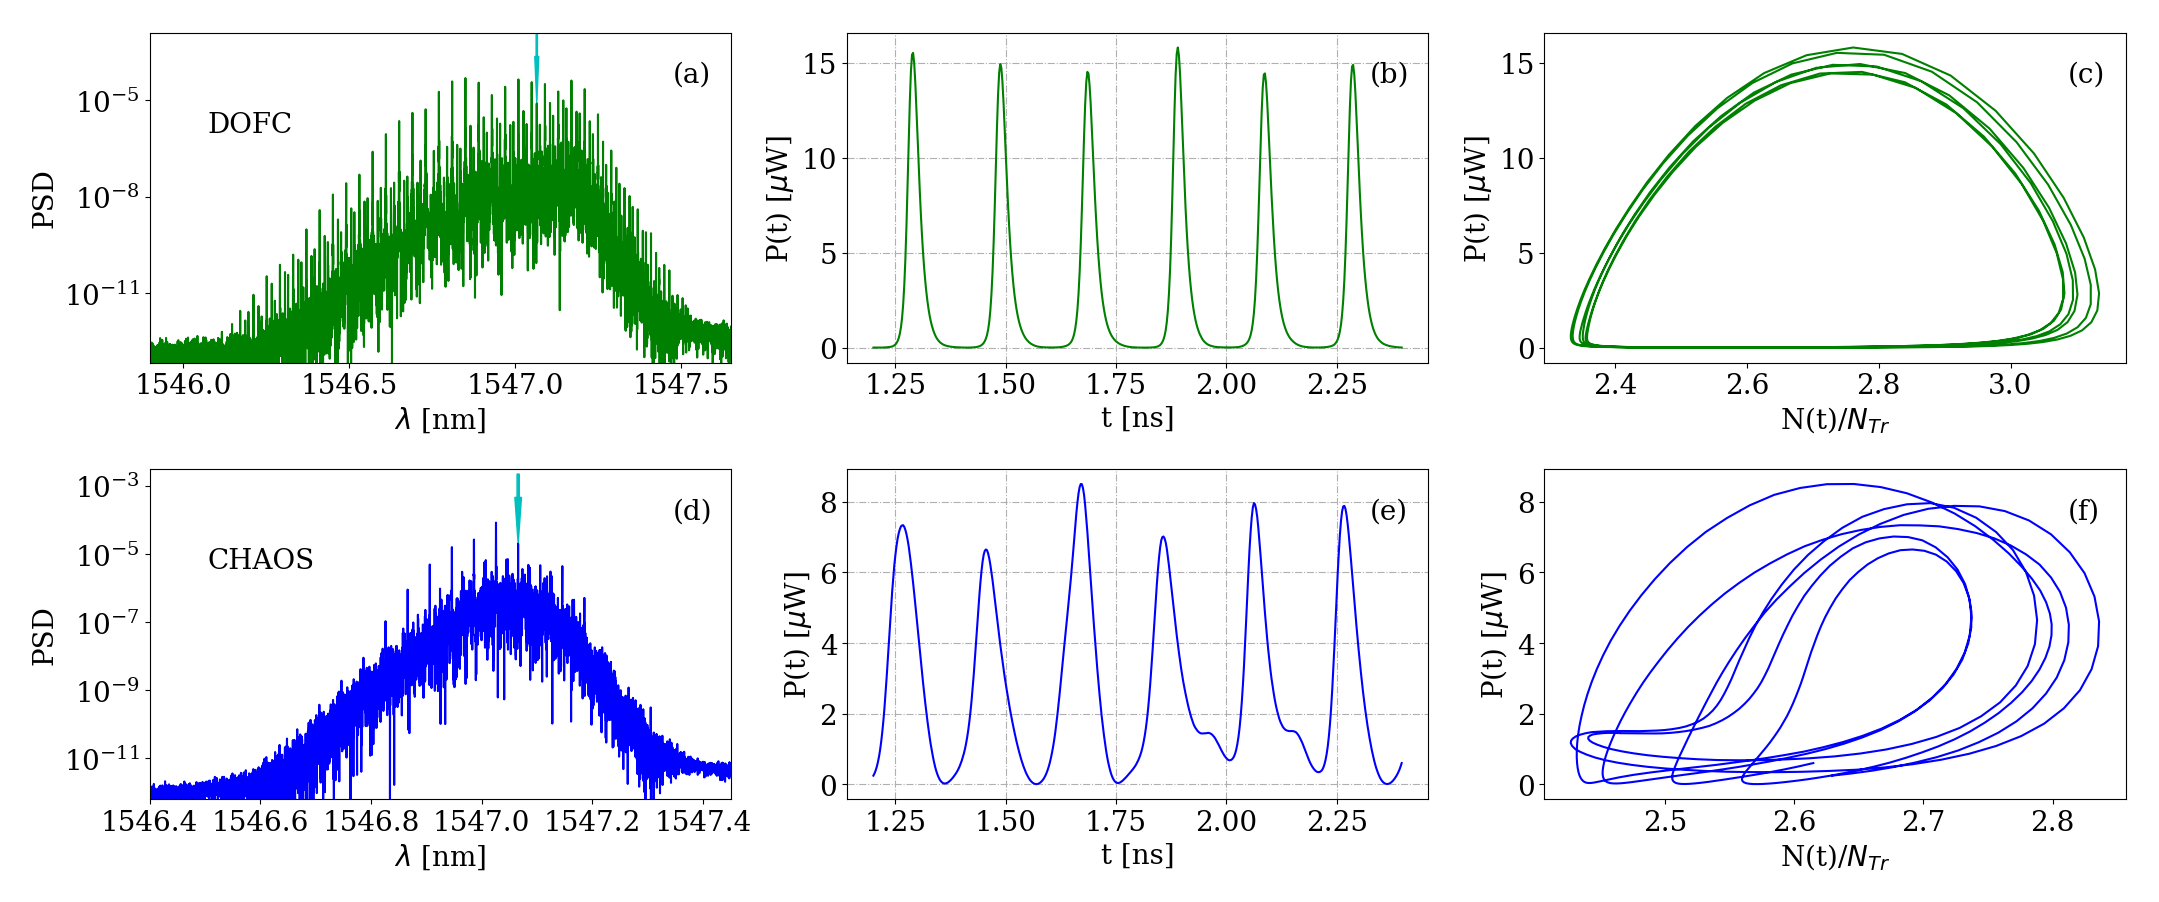
\includegraphics[width=1.0\linewidth]{chaos.png}
		\caption{\label{fig:chaos}Espectros \'opticos, $P(t)$ y proyecci\'on del atractor en el plano ($N(t)$, $P(t)$) del espacio de estados; para $\delta\nu = -2$GHz y $P_{Iny} = 1\;\mu$W (DOFC, naranja) y $300\;\mu$W (CHAOS, azul).}	
	\end{figure}

	Los espectros \'opticos de la Figura \ref{fig:chaos}, con DOFC y CHAOS para $P_{Iny} = 1\;\mu$W y $300\;\mu$W respectivamente, has sido descritos anteriormente. Sin embargo, para la evoluci\'on temporal de $P(t)$ con $P_{Iny} = 1\;\mu$W (Figura \ref{fig:chaos} (b)) se muestran unos picos similares al caso sin inyecci\'on \'optica, al igual que para la proyecci\'on del atractor (Figura \ref{fig:chaos} (c)), debido a que la inyecci\'on es d\'ebil. Adem\'as, se observa que $P(t)$ llega a tomar valores suficientemente pequeños como para que domine la emisión espont\'anea, siendo esta la responsable del mayor ruido en el DOFC del espectro \'optico, y el sistema es m\'as determinista.

	Para la traza temporal de la potencia $P(t)$ con $P_{Iny} = 300\;\mu$W se obtienen picos con una cierta perioicidad, pero con diferencias entre los anchos de los picos, sus formas y, principalmente, sus m\'aximos, obteniendo el comportamiento ca\'otico que se muestra de la proyecci\'on del atractor (Figura \ref{fig:chaos} (f)).
